% This is based on the LLNCS.DEM the demonstration file of
% the LaTeX macro package from Springer-Verlag
% for Lecture Notes in Computer Science,
% version 2.4 for LaTeX2e as of 16. April 2010
%
% See http://www.springer.com/computer/lncs/lncs+authors?SGWID=0-40209-0-0-0
% for the full guidelines.
%
\documentclass{llncs}
\usepackage[T1]{fontenc}
\usepackage[utf8]{inputenc}
\usepackage{lmodern}
\usepackage{mathtools}
\usepackage{minted}
\usepackage{graphicx}
\begin{document}

\title{Japanese Sums in Prolog}
%
\titlerunning{Japanese Sums}  % abbreviated title (for running head)
%                                     also used for the TOC unless
%                                     \toctitle is used
%
\author{Gonçalo Moreno \and João Almeida}
%
\authorrunning{Gonçalo João} % abbreviated author list (for running head)
%

\institute{FEUP, R. Dr. Roberto Frias, 4200-465 Porto}

\maketitle              % typeset the title of the contribution


    
\includegraphics[width=\textwidth]{FEUP.jpg}
  


\begin{abstract}
In this paper we will demonstrate and explain a solution to the number puzzle, Japanese Sums, using Prolog, more specifically the clpfd library, bundled with a SMT solver. Instances of this problem are solved efficiently and fast, on a 3x3 matrix it takes about XX ms. 
\keywords{Prolog. clpfd, Japanese Sums}
\end{abstract}
%
\section{Introduction}
%
\textbf{Japanese Sums} is a logic puzzle more commonly called Number Puzzles or Number. It is a generalization of another more famous number puzzle, \textbf{Kakuro}. Because of this it can be represented as a integer programming problem and it is also NP-complete\cite{np_kakuro}. Brute force or backtracking algorithms are inefficient for solving instances of this problem, but using the Sicstus library "clpfd" we are able solve this problem very efficiently.
% 
\subsection{Rules}
%
The rules are simple, the problem is essentially filling a grid with numbers, so we are initially presented with a empty NxN grid. There is a initial set of numbers where each row or column must use some or all of these numbers. In each row and column are a list of numbers of length L, each block of that row or column must add  
in the correct order to those numbers.

\vspace{1.5cm}
\begin{figure}
  \centering
  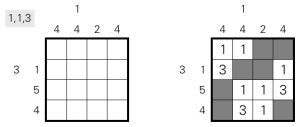
\includegraphics[]{japsum-example.png}
\caption{Instance of Japanese Sum problem.}
  \label{fig:jp_sums}
\end{figure}




\section{Approach}

\subsection{Input}
During development we had multiples ways of starting the program. We decided to choose one that is both simple to the user and requires no parsing. The program is started by the predicate start.

	\begin{minted}{prolog}
start(+SetNumbers, +ColRestrictions, +RowRestrictions, ?Result)
/*Example : start( [0,1,2,3], [[6], [0,3], [3], [4,2]],
[[3,1], [1,5], [2,1], [5]], Result). */
	\end{minted}
    
\subsection{Decision Variables}

The variables needed to be labeled represent each cell of a NxN grid. They are positive integer numbers with exception of the empty cells that are represented internally by -1.

Result is the output and the decision variables.

\subsection{Constraints}

The hardest part of solving this puzzle is adding the restrictions to the solver. 

\subsubsection{Set Restrictions}

All the numbers in a row or column must be drawn from the a initial set. We tackle

\subsection{Search Strategy}

\section{Solution Presentation}

The solution is presented in the form of a NxN grid/matrix where the blocks are separated by empty cells which are represented by "\#". The restrictions are also shown.

\vspace{1.5cm}
\begin{figure}
  \centering
  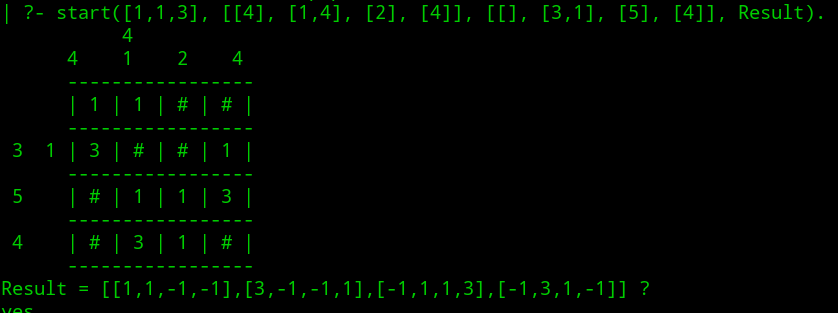
\includegraphics[width=\textwidth]{solution-example.png}
\caption{Presentation of a solution.}
  \label{fig:ex_sol_jp_sums}
\end{figure}



\section{Results}
We used our program to run a variety of Puzzles from sizes 3 up to 8. We used sicstus timer to measure the results. The timer wasn't very precise for puzzles of size 3 and 4. We also didn't test with puzzles from size 9 or more because we couldn't find ones bigger than 8 and also the ones of size 8 took a lot of time to measure. Below is a graph of the running times.


\begin{figure}
  \centering
  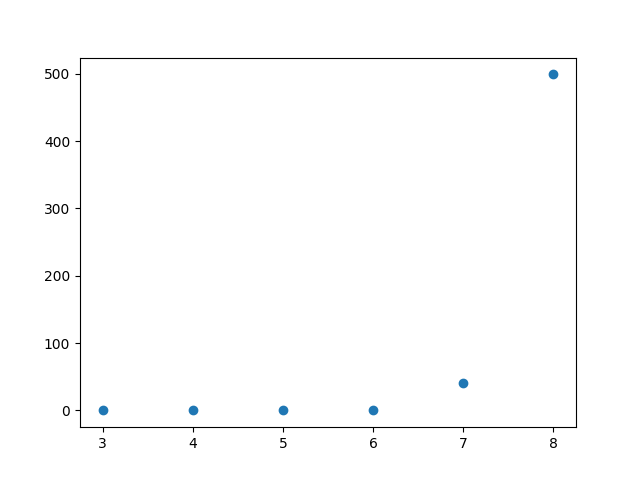
\includegraphics[width=\textwidth*2/3]{times2.png}
\caption{Running times vs Size.}
  \label{fig:times}
\end{figure}

The tests were ran on a machine with a i7 4770k, 16GB of Ram and running Arch Linux 4.13.12.

As we can see from the graph the running times increase exponentially with the size of the grid. This is expected as with any NP-Complete Problem.
\linebreak

In order to try to determine what would be the running times for puzzles of size higher than 8 we used exponential fitting and we got a curve of :

\begin{equation}
y = 5.347875472 \times 10^{-7} \times e^{2.582101184 x}
\end{equation}

Extrapolating for size of 9 we get about 6617s which is about 2 hours of running time. For size of 10 its 87519s or about 24 hours. 

\subsection{Generating Puzzles}

We have also developed a predicative that will generate puzzles, you only need to specify the set numbers and size and it will generate a puzzle and solve it. It takes a long time to generate one for N > 6.

	\begin{minted}{prolog}
	generate_puzzle(+SetNumbers, +Size, ?Result)
	\end{minted}

It randomly generates the size of the restrictions for both the columns and rows and then randomly generates lists of numbers accordingly to the size and the input numbers.

\section{Conclusions and Future Work}
Creating this program was simple, we didn't have to come up with a algorithm to solve the puzzle or any complicated mathematics. We simply "stated" the problem in Prolog and use the solver available in the clpfd library to solve it.
\\~\\

From the results section it is clear that solving instances of this problem is still very demanding even with a efficient SMT solver. We could make the program run faster by adding further restrictions. The ones that we add are the ones specified by the rules, we could probably find ones that aren't so explicit and doing so we could reduce the running times. 
\\~\\

The Puzzle generator needs to be improved as it currently stands it only generates puzzles up to size 6 and the ones that are generated could have more restrictions. We need to better implement the mathematics behind the generation of the numerical value of each restriction.

%
% ---- Bibliography ----
%
\begin{thebibliography}{5}
%
\bibitem {np_kakuro}
Takahiro, S. (2001): The complexities of puzzles, cross sum and their another solution problems (ASP). Thesis for BSc, Department of Information Science, University of Tokyo.



\end{thebibliography}

\end{document}
